\subsection{Investigating gated recurrent networks for speech synthesis \cite{Wu2016Investigating}}

Recently, \emph{recurrent neural networks (RNNs)} have re-emerged as a potential acoustic model for \emph{statistical parametric speech synthesis (SPSS)}. This paper attempts to answer two questions: 1) why do LSTMs work well as a sequence model for SPSS; 2) which component of the LSTM unit is most important. It presents a visual analysis along the experiments, resulting in a simplified architecture.

The goal of the paper is to reach a better understanding of the ``black-box'' LSTM architecture. First, it gives an analysis of the forget gate and memory cell in the LSTM architecture. Specifically, it visualises the activation of the forget gate to understand when the forget gate resets the memory cell state, and how the forget gate relates to speech structure. Second, it analyses the importance of each LSTM component (e.g., input gate, output gate, forget gate), and proposes a simplified architecture.

To assess the importance of each component, the paper starts with four variants of the LSTM architecture: 1) No Peep-holes (NPH): Set the peep-hole connections $p^i, p^o, p^f$ to zeros. 2) No input gate (NIP): Set the input gate to 1 ($i_t = 1$). 3) No forget gate (NFG): Set the forget gate to 1 ($f_t = 1$). 4) No output gate (NOG):  Set the output gate to 1 ($o_t = 1$).

\begin{figure}[htbp]
  \centering
  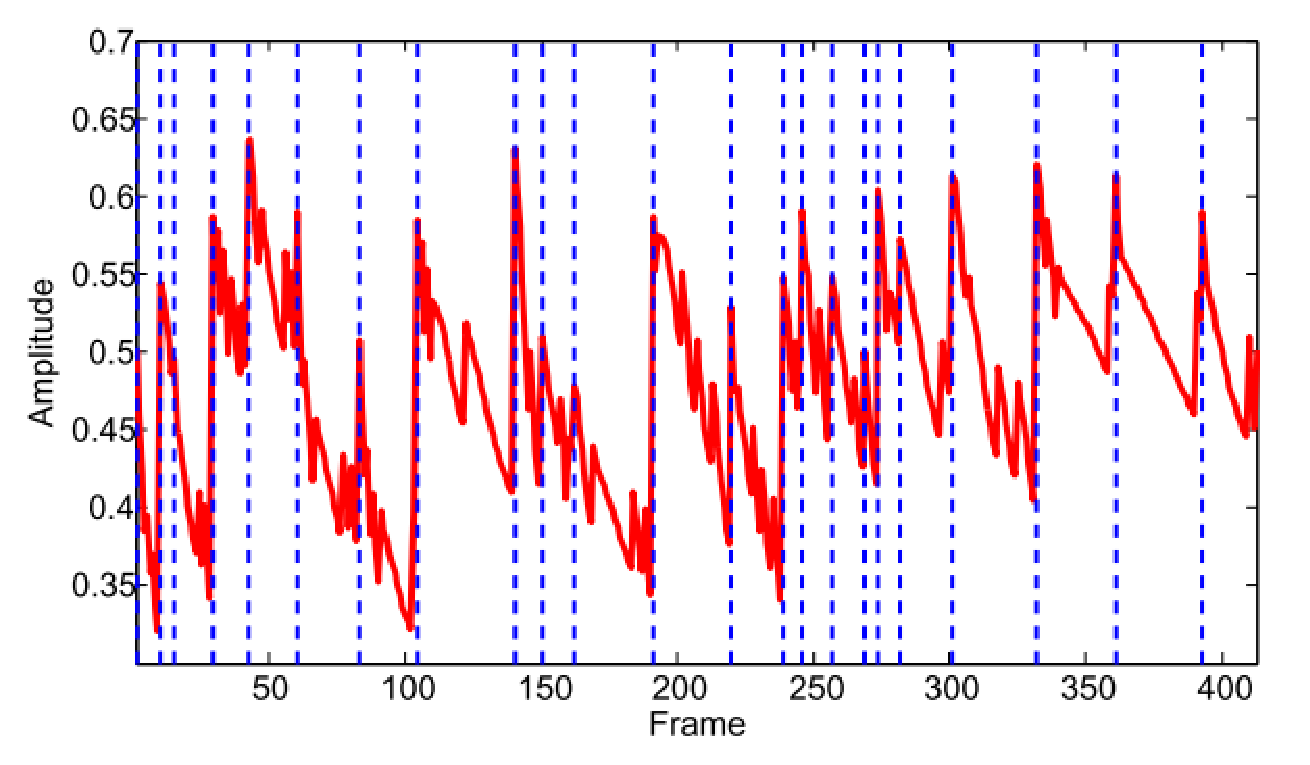
\includegraphics[width=.5\linewidth]{10_3_acu1}\\
  \caption{Averaged activations of all forget gates}\label{fig:acu1}
\end{figure}

\begin{figure}[htbp]
  \centering
  % Requires \usepackage{graphicx}
  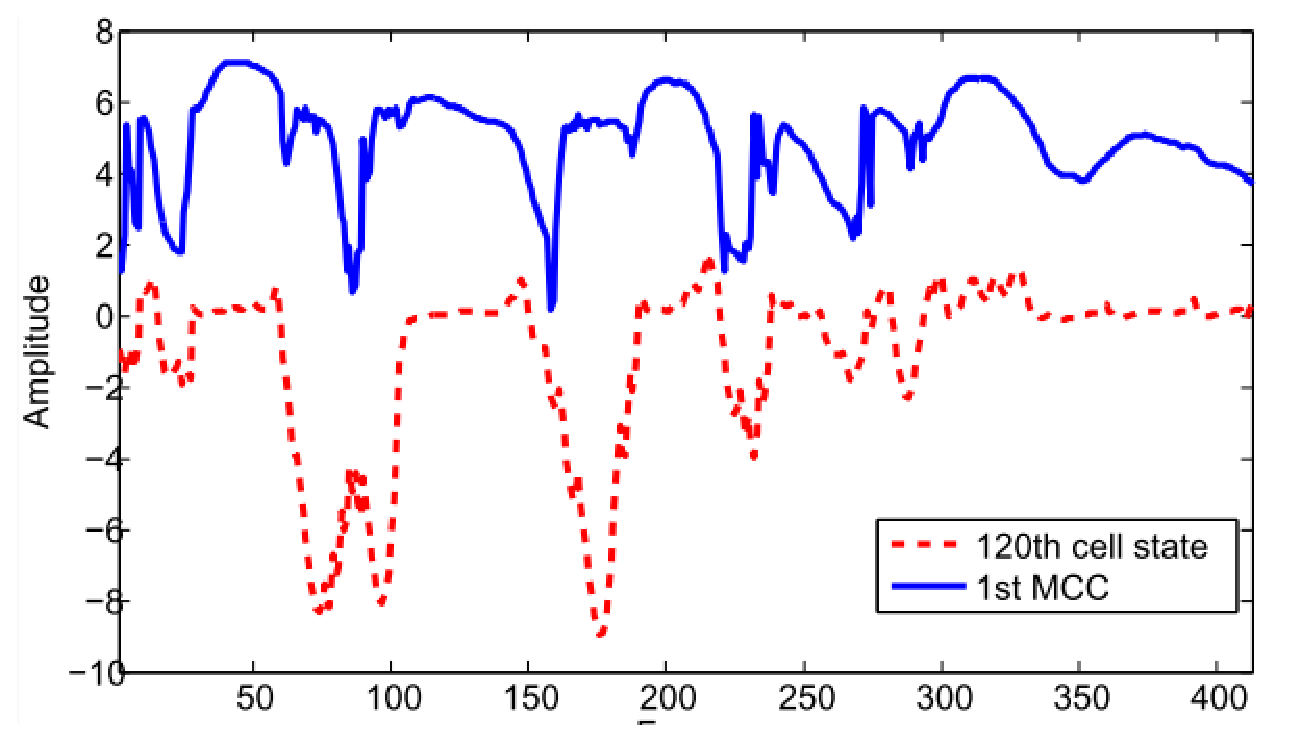
\includegraphics[width=.5\linewidth]{10_3_acu2}\\
  \caption{Comparison between the Mel-Cepstral Coefficient (MCC) trajectory and a cell state}\label{fig:acu2}
\end{figure}

The first step of the analysis is to visualise the forget gate and cell state, which are thought to be the two most important components in modelling long-term temporal structure. The averaged activations over the 256 units of the forget gate are presented in Figured \ref{fig:acu1}. It can be observed that the peaks of the forget gate activation trajectory have a strong correspondence with the phoneme boundaries. The memory cell should store the trend of the trajectory to be predicted, and a comparison between the relation is presented in Figure \ref{fig:acu2}.

The objective experiment compares the standard LSTM with different variations. The results show that the NFG system increases distortion considerably, which implies that the forget gate is the most important. Based on this observation, the paper proposes a simplified LSTM structure, which removes output gates and peep-hole connections, and replaces the input gate by the forget gate. The other experimental results also shows that the simplified LSTM is as good as any other systems.

Remark: This paper provides a detailed analysis of the performance of different components of the LSTM unit. In many occasions, we tend to use network architectures like LSTM as black boxs - we believe that they would work well because they are successful in other tasks. This paper reminds us that it is still necessary to look into why a network works on a specific problem. This may bring us deeper insight, and probably result in a better architecture. 